\chapter{Landasan Teori}
\label{chap:LandasanTeori}

%\section{MySQL Spatial Extensions}
%\label{sec:mysqlspatial}
%MySQL merupakan sistem manajemen basisdata yang mempunyai performa tepercaya, handal, dan mudah penggunaannya. Penggunaan MySQL dipilih untuk aplikasi berbasis web. Bentuk basisdata MySQL adalah relasional, yang berarti tabel-tabel yang terdapat pada MySQL saling berhubungan. Server MySQL berada pada klien / server atau pada sistem yang tertanam pada aplikasi.
%
%MySQL mengimplementasikan ekstensi spasial, yaitu MySQL dengan tipe geometri. MySQL dengan tipe geometri mempunyai kolom khusus dengan tipe geometri dan mempunyai fungsi untuk membuat dan menganalisis nilai geometri. Ekstensi spasial MySQL memungkinkan generasi, penyimpanan, dan analisis fitur geometris :
%
%\begin{itemize}
%	\item Tipe data untuk merepresentasikan nilai spasial.
%	\item Fungsi untuk manipulasi nilai spasial.
%	\item Pengindeksan spasial untuk mempercepat waktu akses ke kolom spasial.
%\end{itemize}
%
%Fitur geografi dapat berupa apapun di dunia yang mempunyai lokasi. Fitur geografi dapat berupa:
%
%\begin{itemize}
%	\item Sebuah entitas, seperti gunung, laut, dan kota.
%	\item Sebuah ruang, seperti batas kota dan daerah tropis.
%	\item Sebuah definisi tempat, seperti perempatan jalan.
%\end{itemize}

\section{Play Framework}
\label{sec:play}
\subsection{Struktur Play Framework}
\play \cite{playforjava} merupakan \textit{framework} untuk aplikasi web dengan menggunakan bahasa Java dan Scala. \play tidak sepenuhnya menggunakan bahasa Java, tetapi ada juga bahasa Scala. Terdapat bahasa Scala bukan berarti harus mempelajari bahasa Scala karena dalam Play 2 dilengkapi dengan Java API yang komplit, memberikan opsi untuk memilih bahasa pemrograman yang cocok. \play mempunyai antarmuka yang sederhana, nyaman, fleksibel, dan kuat. Referensi yang digunakan membahas \play 2.2, sedangkan versi \play yang dipakai dalam penelitian ini adalah versi 2.4. Ada sedikit perbedaan sintaks yang akan dijelaskan pada bagian yang berbeda.
Beberapa fitur utama yang membuat \play produktif dan penggunaan yang nyaman:

\begin{enumerate}
	\item Penggunaan \play sederhana.
	\item Konfigurasi skema URL aplikasi deklaratif.
	\item Pemetaan type-safety.
	\item \play menyediakan contoh sintaks type-safety.
	\item Arsitektur yang mencakup teknologi HTML5.
	\item Kode langsung aktif berubah ketika memuat kembali halaman web.
	\item Fitur \textit{full-stack web-framework}, termasuk \textit{persistence}, keamanan, dan \textit{internationalization}. \textit{Persistence} adalah ide yang menggunakan koneksi TCP yang sama untuk mengirim dan menerima beberapa HTTP \textit{requests/responses} tanpa membuka TCP baru untuk setiap \textit{requests/responses} dengan tujuan untuk meningkatkan kinerja HTTP.
	\item Mendukung aplikasi \textit{event-driven} dan dinamis.
\end{enumerate}

\play memiliki struktur yang dapat dilihat pada gambar \ref{fig:2_play_struktur}.

\begin{figure}[H]
	\centering
	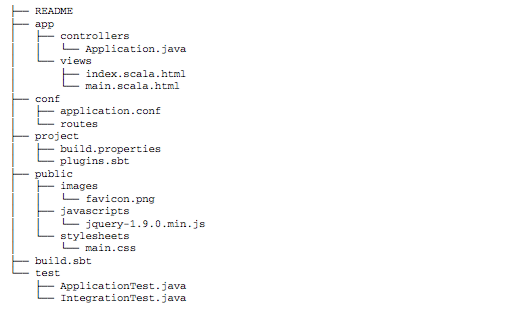
\includegraphics[scale=0.7]{Gambar/play-struktur}
	\caption{Struktur Play Framework} 
	\label{fig:2_play_struktur}
\end{figure}

\subsubsection{Direktori conf.}
Konfigurasi \play terdapat pada direktori \textit{conf}. Dalam direktori \textit{conf}, terdapat file \textit{application.conf} dan \textit{routes}. File \textit{application.conf} mengandung informasi data konfigurasi aplikasi, seperti \textit{logging}, koneksi basis data, dan port berapa server berjalan. File \textit{routes} menentukan \textit{routes} aplikasi, yaitu pemetaan dari URL HTTP ke kode aplikasi. Setiap \textit{routes} memiiki tiga bagian, yaitu HTTP \textit{method}, URL \textit{path}, dan \textit{action method}. HTTP \textit{method} merupakan metode yang dipakai dalam pengiriman HTTP. URL \textit{path} adalah URL yang dipakai untuk mengakses halaman. \textit{Action method} merupakan metode  yang dipanggil ketika mengakses halaman pada URL \textit{path}. Sebagai contoh dapat dilihat pada \ref{fig:2_play_routes}, HTTP \textit{method} yang dipakai pada URL /list adalah HTTP \textit{method} GET dan akan memanggil \textit{method} list pada kelas Products di controllers.

\begin{figure}[H]
	\centering
	
\includegraphics[scale=0.7]{Gambar/play-routes}
	\caption{Contoh \textit{Routes}} 
	\label{fig:2_play_routes}
\end{figure}

\subsubsection{Direktori public}
Direktori \textit{public} mengandung semua sumber daya yang disediakan langsung tanpa melalui proses terlebih dahulu. Direktori \textit{public} biasanya mengandung file gambar, \textit{stylesheets}, JavaScript, dan halaman statis HTML. Contoh direktori \textit{public} dapat dilihat pada gambar \ref{fig:2_play_struktur}.
%
%\begin{figure}[H]
%	\centering
%	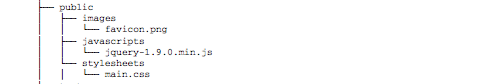
\includegraphics{Gambar/play-public}
%	\caption{Contoh Direktori \textit{public}} 
%	\label{fig:2_play_public}
%\end{figure}

\subsubsection{Direktori app.}
Direktori \textit{app} merupakan direktori utama pada aplikasi. Direktori \textit{app} berisi kode aplikasi dan berbagai kebutuhan untuk menyusun aplikasi, seperti sumber file Java dan file \textit{template}. Contoh direktori \textit{app} pada saat pertama kali membuat aplikasi Play dapat dilihat pada gambar \ref{fig:2_play_struktur}. 

Dalam \textit{controller}, terdapat file Application.java yang berisi kode Java untuk memuat halaman \textit{view}. \textit{Controller} adalah kelas untuk menerima HTTP \textit{request} dan mengembalikan nilai dari HTTP \textit{request} berupa view. Ada dua file template, yaitu index.scala.html dan main.scala.html yang berfungsi untuk menentukan halaman HTML yang akan dimuat. Semua konten yang dihasilkan di server dan dikirimkan ke klien seperti halaman HTML disebut \textit{view}. View dapat menerima parameter yang didefinisikan pada template view. Contoh view dengan menerima parameter berupa String dapat dilihat pada kode listing \ref{lst_2_view}. \textit{Method} pada \textit{Controller} menghasilkan hasil berupa \textit{Result} yang berupa \textit{view} dengan memberi parameter "Hello World". \textit{Method} pada \textit{controller} dan \textit{view} dihubungkan melalui pendefinisian pada \textit{routes}. Sebagai contoh pada kode listing \ref{lst_2_controller}, \textit{method ok} membangun HTTP \textit{response} yang mengandung \textit{response body} sebagai hasil dari \textit{template list}. \textit{Method ok} menerima \textit{parameter} berupa "Hello World". Pada \cite{playforjava}, hasil Result dalam \verb!static!, tetapi pada \play 2.4 \verb!static! dihilangkan.
% Products pada \textit{parameter ok} menyerahkan semua data kepada \textit{model}, yaitu kelas Product dan merepresentasikan data ke \textit{view}, yaitu \textit{template list}. \textit{Method} list() mengembalikan \textit{view products} dengan mengirimkan \textit{parameter} berupa \textit{list of products}. 

\begin{lstlisting}[caption=Contoh View,label = {lst_2_view},language=Java]
@(title: String)

	<!DOCTYPE html>

	<html>
    		 <head>
       	 <title>@title</title>
       	 <link rel="stylesheet" media="screen" href="@routes.Assets.at("stylesheets/main.css")">
       	 <link rel="shortcut icon" type="image/png" href="@routes.Assets.at("images/favicon.png")">
        	<script src="@routes.Assets.at("javascripts/jquery-1.9.0.min.js")" type="text/javascript"></script>
    		</head>
    		<body>
        		@title
    		</body>
	</html>
\end{lstlisting}


\begin{lstlisting}[caption=Contoh Controller,label = {lst_2_controller},language=Java]
	public Result index() {
        return ok(index.render("Hello World"));
    }
\end{lstlisting}

Beberapa alternatif hasil Results, yaitu:
\begin{enumerate}
	\item \textbf{Method ok} 
	Method yang berfungsi untuk mengembalikan Result dengan kode \textit{HTTP Response} 200 atau sukses dalam mengirim \textbf{HTTP Request}.
	\item \textbf{Method notFound} 
	Method yang berfungsi untuk mengembalikan Result dengan  kode \textit{HTTP Response} 404 atau tidak ada halaman yang dituju.
	\item \textbf{Method badRequest} 
	Method yang berfungsi untuk mengembalikan Result dengan kode \textit{HTTP Response} 400 atau adanya kesalahan masukan pengguna.
	\item \textbf{Method internalServerError}
	Method yang berfungsi untuk mengembalikan Result dengan kode \textit{HTTP Response} 500 atau adanya kesalahan pada server.
	\item \textbf{Method status}
	Method yang berfungsi untuk mengembalikan Result dengan kode \textit{HTTP Response} yang dapat ditentukan sendiri beserta pesannya.
	\item \textbf{Method redirect}
	Method yang berfungsi untuk mengembalikan Result untuk mengalihkan halaman.
\end{enumerate}

\subsection{Body Parsers}
\textit{Body parsers} bertugas untuk melakukan pemetaan \textit{request body} menjadi objek. Setiap \textit{action method} POST dan PUT mengandung \textit{body}. Jumlah \textit{body} dapat satu atau banyak, dan dapat berupa XML, JSON, data biner, atau dapat berupa apapun sesuai Content-Type pada \textit{header request}. \textit{Body parsers} akan menguraikan \textit{body} menjadi objek Java. \textit{Body parsers} mengubah \textit{request} menjadi objek yang dapat digunakan oleh komponen Play. Karena \textit{body} JSON dan \textit{body} XML berbeda penguraiannya, Play menggunakan \textit{body parsers} yang berbeda pula implementasinya. Berbeda Content-Type pada \textit{header request}, \textit{body parsers} spesifik dapat mengubah data yang masuk menjadi sesuatu yang dapat dimengerti oleh Play. Ilustrasi dapat dilihat pada gambar \ref{fig:2_play_bodyparsers}.

\begin{figure}[H]
	\centering
	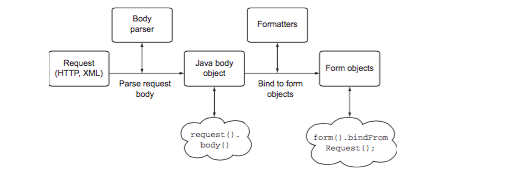
\includegraphics[scale=0.7]{Gambar/play-bodyparsers}
	\caption{Interaksi \textit{Body Parsers} dengan \textit{Request}} 
	\label{fig:2_play_bodyparsers}
\end{figure}

%\section{Kode KIRI (PHP)}
%\label{sec:kodeKIRI}


\subsection{Internationalization}
Pengguna aplikasi mungkin berasal dari beda negara dan bahasa, juga punya format yang berbeda untuk tanggal, angka, dan waktu. Kombinasi dari bahasa aturan format disebut \textit{locale}. Adaptasi program untuk berbeda \textit{locale} disebut \textit{internationalization (i18n)} atau \textit{localization (l10n)}. Perbedaan \textit{internationalization} dan \textit{localization} adalah \textit{internationalization} melakukan \textit{refactor} untuk menghapus kode lokal dari aplikasi, sedangkan \textit{localization} membuat versi lokal dari aplikasi. Program yang sudah diproses Internationalization mempunyai karakteristik:

\begin{itemize}
	\item Dengan penambahan data lokalisasi, eksekusi yang sama dapat dijalankan di seluruh dunia.
	\item Unsur tekstual, seperti pesan status dan komponen GUI, tidak ada \textit{hard-code} dalam program. Sebaliknya, pesan status dan komponen GUI disimpan di luar \textit{source code} dan diambil secara dinamis.
	\item Dengan adanya bahasa baru, program tidak perlu dikompilasi ulang.
	\item Data culturally-dependent, seperti tanggal dan mata uang, tampil dalam format yang sesuai dengan wilayah pengguna.
	\item Internationalization dapat dilakukan proses lokalisasi dengan cepat.
\end{itemize}

Untuk mendukung beberapa bahasa dalam Play, membuat kunci pesan yang dipetakan pesan sesungguhnya pada file pesan. Pesan ini dimuat dalam file messages.LANG dimana LANG merupakan bahasa yang dipakai. Sebagai contoh, terdapat dua bahasa yang dipakai pada aplikasi, yaitu Bahasa Inggris dan Bahasa Indonesia seperti pada kode listing \ref{lst_2_i18n_en} dan \ref{lst_2_i18n_id}

\begin{lstlisting}[caption=Contoh messages.en untuk i18n,label = {lst_2_i18n_en},language=Java]
	from = From:
	ph_from = e.g. Stasiun
	ph_to = e.g. Monas,Jakarta
	find = Find!
	to = To:
\end{lstlisting}

\begin{lstlisting}[caption=Contoh messages.id untuk i18n,label = {lst_2_i18n_id},language=Java]
	from = Dari:
	ph_from = misal: Stasiun
	ph_to = misal: Monas, Jakarta
	find = Cari!
	to = Ke:
\end{lstlisting}

Play harus mengetahui bahasa apa saja yang ada pada aplikasi sesuai dengan file messages.LANG. Untuk itu, daftarkan bahasa pada application.conf seperti pada kode listing \ref{lst_2_conf_i18n}. Pada \cite{playforjava}, konfigurasi bahasa dalam satu String. Tetapi pada \play 2.4 konfigurasi bahasa dalam bentuk array of String.

\begin{lstlisting}[caption=Konfigurasi Bahasa i18n,label = {lst_2_conf_i18n},language=Java]
	application.langs=["en","id"]
\end{lstlisting}


	
	
\section{OpenLayers}
\label{sec:openlayers}
OpenLayers \cite{openlayersbook} merupakan \textit{library} yang memiliki performa tinggi dan fitur yang dikemas untuk kebutuhan menampilkan peta menggunakan JavaScript. Dalam pengembangan aplikasi yang menggunakan fitur peta, tugas yang paling penting dan utama adalah membuat peta tersebut. Peta menjadi inti untuk menambahkan dan menampilkan data. Fitur yang terdapat pada OpenLayers adalah:

\begin{itemize}
\item \textit{Tiled Layers}\\
			OpenLayers dapat menggunakan banyak \textit{map provider}, seperti OSM, Bing, MapBox, Stamen, MapQuest, dan berbagai sumber lain yang dapat ditemukan. Dengan menggunakan OpenLayers, tidak perlu menulis ulang kode yang sudah ada dan dapat mengganti kapanpun sumber \textit{map provider} yang ingin digunakan.
	\item \textit{Vector Layers}\\
			OpenLayers dapat mengubah data vektor dari berbagai tipe sumber, seperti GeoJSON, TopoJSON, KML, dan GML.
	\item Cepat dan Siap untuk Perangkat \textit{Mobile}\\
			OpenLayers mendukung perangkat \textit{mobile}. OpenLayers dapat membangun profil kustom yang berisi komponen yang dibutuhkan saja.
	\item Mudah menyesuaikan peta dan \textit{cutting edge}\\
			OpenLayers menyesuaikan peta WebGL, Canvas 2D, dan semua kelebihan dari HTML 5. Atur tampilan peta dengan mengubah langsung CSS.
\end{itemize}

Modul OpenLayers yang dipakai dalam penelitian ini adalah:
\begin{itemize}
	\item 	Bing Maps untuk menampilkan peta menggunakan Bing. KIRI menggunakan \textit{map provider} Bing Maps sebagai peta pada halaman utama KIRI. 
	\item Draw untuk menggambar poin pada peta. Saat peta KIRI menangkap \textit{event mouseclick}, muncul poin yang berupa kustom gambar pada peta KIRI sebagai asal tempat dan tujuan. 
\end{itemize}

\subsection{Bing Maps}
Peta yang digunakan merupakan Bing Maps dari Microsoft. Jika ingin menggunakan Bing Maps pada Openlayers, harus mendapatkan kunci yang didapat dari Bing Maps serta memilih tipe peta yang akan ditampilkan. Sebagai contoh pada kode listing \ref{lst_2_ol_bing}.

\begin{lstlisting}[caption=Penggunaan Bing Maps pada Openlayers,label = {lst_2_ol_bing},language=Java]
var mapLayer = new ol.layer.Tile(
{
	source : new ol.source.BingMaps(
    	{
     	key : 'AuV7xXD6_UMiQ5BLoZr0xkpjLpzWqMT55772Q8XtLIQeuDebHPKiNXSlZXxEr1GA',
         imagerySet : 'Road'
     })
});
\end{lstlisting}

\subsection{Draw Poin}
Pada peta KIRI, pengguna dapat memilih tempat awal dan tujuan dengan memasukkan nama tempat atau memilih tempat pada peta. Pada Openlayers, disediakan fitur untuk menangani kursor klik pengguna. Pertama menentukan gambar yang akan ditampilkan pada peta seperti pada kode listing \ref{lst_2_ol_image}. Setelah itu, menggambar pada peta seperti pada figur \ref{lst_2_ol_map}.


\begin{lstlisting}[caption=Menentukan gambar yang akan dipakai pada peta,label = {lst_2_ol_image},language=Java]

	
	var markers = {start: null, finish: null};
	
	var inputVectorSource = new ol.source.Vector();

	markers['start'] = new ol.Feature(
	{
		geometry: new ol.geom.Point(event.coordinate)
	})
	
	markers['start'].setStyle(new ol.style.Style(
	{
		image: new ol.style.Icon({
			src: '/assets/images/start.png',
			anchor: [1.0, 1.0]
		})
	}));
	
	inputVectorSource.addFeature(markers['start']);
	
	
\end{lstlisting}


\begin{lstlisting}[caption=Menambahkan vektor pada peta,label = {lst_2_ol_map},language=Java]
	
var map = new ol.Map({
    target: 'map',
    layers : [ mapLayer, new ol.layer.Vector({source: inputVectorSource}), new ol.layer.Vector({source: resultVectorSource}) ],
    view: new ol.View({
        center: ol.proj.fromLonLat([107.60981,-6.91474]),
        zoom: 12
    })
});
		
\end{lstlisting}

\section{Zurb Foundation}
\label{sec:zurbfoundation}
%Zurb Foundation \cite{zurbfoundation} merupakan \textit{framework Front-End} yang responsif dan terdepan untuk membuat tampilan halaman web. Halaman web yang menggunakan Zurb Foundation sudah \textit{mobile-friendly} dan siap untuk diubah sesuai dengan keinginan. Fitur yang dimiliki Zurb Foundation adalah:
%
%\begin{itemize}
%	\item Zurb Foundation memuat halaman web menjadi cepat.
%	\item Zurb Foundation melakukan optimasi halaman web dengan memilih bagian halaman web untuk dimuat berdasarkan tipe perangkat pengguna.
%	\item Zurb Foundation lebih cepat dalam menulis kode.
%	\item Zurb Foundation cepat untuk dipelajari.
%%	\item Zurb Foundation merupakan pilihan profesional bagi perusahaan, desainer, dan pengembang.
%	\item Zurb Foundation adalah \textit{framework} yang responsif.
%	\item Zurb Foundation mempunyai tampilan yang baru dan modern.
%\end{itemize}

Zurb Foundation \cite{zurbfoundationbook} merupakan sebuah \textit{toolkit} yang membantu untuk desain dan mengembangkan sebuah halaman \textit{web}. Zurb Foundation menggunakan sistem \textit{grid}, banyak komponen CSS serta JavaScript. 

\subsection{Sistem Grid}
Sistem \textit{grid} pada Zurb Foundation adalah semacam \textit{spreadsheet}, graf atau tabel yang digunakan untuk mengatur tampilan HTML. Gambaran sistem \textit{grid} dapat dilihat pada gambar \ref{fig:2_zurb_grid_blank}.

\begin{figure}[H]
	\centering
	
\includegraphics[scale=0.5]{Gambar/zurb-gridblank}
	\caption{Sistem \textit{grid} kosong sebelum memulai desain.} 
	\label{fig:2_zurb_grid_blank}
\end{figure}

Setiap sel merupakan area konten yang dapat digabung dengan sel lain yang bersebelahan untuk memperbesar area konten. Sel yang digunakan pada Zurb Foundation adalah 12 sel pada setiap baris. Gambaran pembagian sel pada Zurb Foundation dapat dilihat pada gambar \ref{fig:2_zurb_grid}.

\begin{figure}[H]
	\centering
	
\includegraphics[scale=0.5]{Gambar/zurb-grid}
	\caption{Contoh pembagian sistem \textit{grid}.} 
	\label{fig:2_zurb_grid}
\end{figure}

Komponen Foundation adalah kode CSS  yang membantu untuk desain dan merepresentasikan konten halaman \textit{web}. Dengan menggunakan komponen Foundation, tidak perlu desain sendiri dari awal. CSS pada Foundation juga dapat dikustomisasi sesuai dengan kebutuhan. Jika ingin menggunakan komponen Foundation, kita hanya perlu menggunakan tag class pada elemen yang diinginkan. Contoh penggunaaan komponen Foundation dapat dilihat pada figur \ref{lst_2_zurb_contoh}.

\begin{lstlisting}[caption=Menggunakan kelas yang sudah disediakan dari Foundation,label = {lst_2_zurb_contoh}]
	<img class="show-for-small" src="./images/little.png"/>
\end{lstlisting}

\section{Chrome DevTools}
\label{sec:devtools}
Chrome DevTools\cite{devtools} merupakan perangkat untuk memperhatikan dan melakukan \textit{debugging} halaman web yang terdapat pada \textit{browser} Google Chrome. DevTools dapat digunakan secara efisien untuk memeriksa tampilan, mengatur \textit{breakpoints} JavaScript, dan optimasi kode. DevTools dapat diakses dengan melakukan klik kanan pada halaman web lalu klik periksa elemen. DevTools disusun dalam beberapa panel \textit{task-orientated}. Beberapa panel tersebut adalah:

\begin{enumerate}
	\item \textbf{Elements}, untuk memeriksa, melihat, dan mengubah tampilan halaman web.
	\item \textbf{Network}, untuk memantau aktivitas jaringan pada halaman web secara \textit{real-time}.
	\item \textbf{Sources}, untuk melakukan \textit{debugging} pada JavaScript dengan menentukan \textit{breakpoints}.
	\item \textbf{Timeline}, untuk merekam dan analisis aktivitas halaman web.
	\item \textbf{Profiles}, untuk menggambarkan waktu eksekusi dan penggunaan memori dari halaman web.
	\item \textbf{Resources}, untuk memeriksa sumber daya halaman web, seperti basis data, \textit{cookies}, \textit{cache}, gambar, dan tampilan halaman web.
	\item \textbf{Console}, untuk mencatat informasi diagnostik pada proses pengembangan serta menyediakan \textit{prompt shell} yang dapat digunakan untuk interaksi dengan dokumen dan DevTools.
\end{enumerate}

\subsection{Elements}
Panel Elements dapat memperlihatkan struktur halaman web dalam bentuk \textit{Document Object Model} (DOM), dan dapat mengubah elemen DOM dengan cepat. DOM adalah struktur logis dokumen serta cara dokumen diakses dan diubah \footnote{\url{http://www.w3.org/TR/DOM-Level-2-Core/introduction.html}, diakses 2 Oktober 2015}. Sebagai contoh pada gambar \ref{fig:2_devtools_elements}, pemeriksaan elemen akan memperlihatkan dua bagian, yaitu DOM dan CSS yang digunakan pada DOM.

\begin{figure}[H]
	\centering
	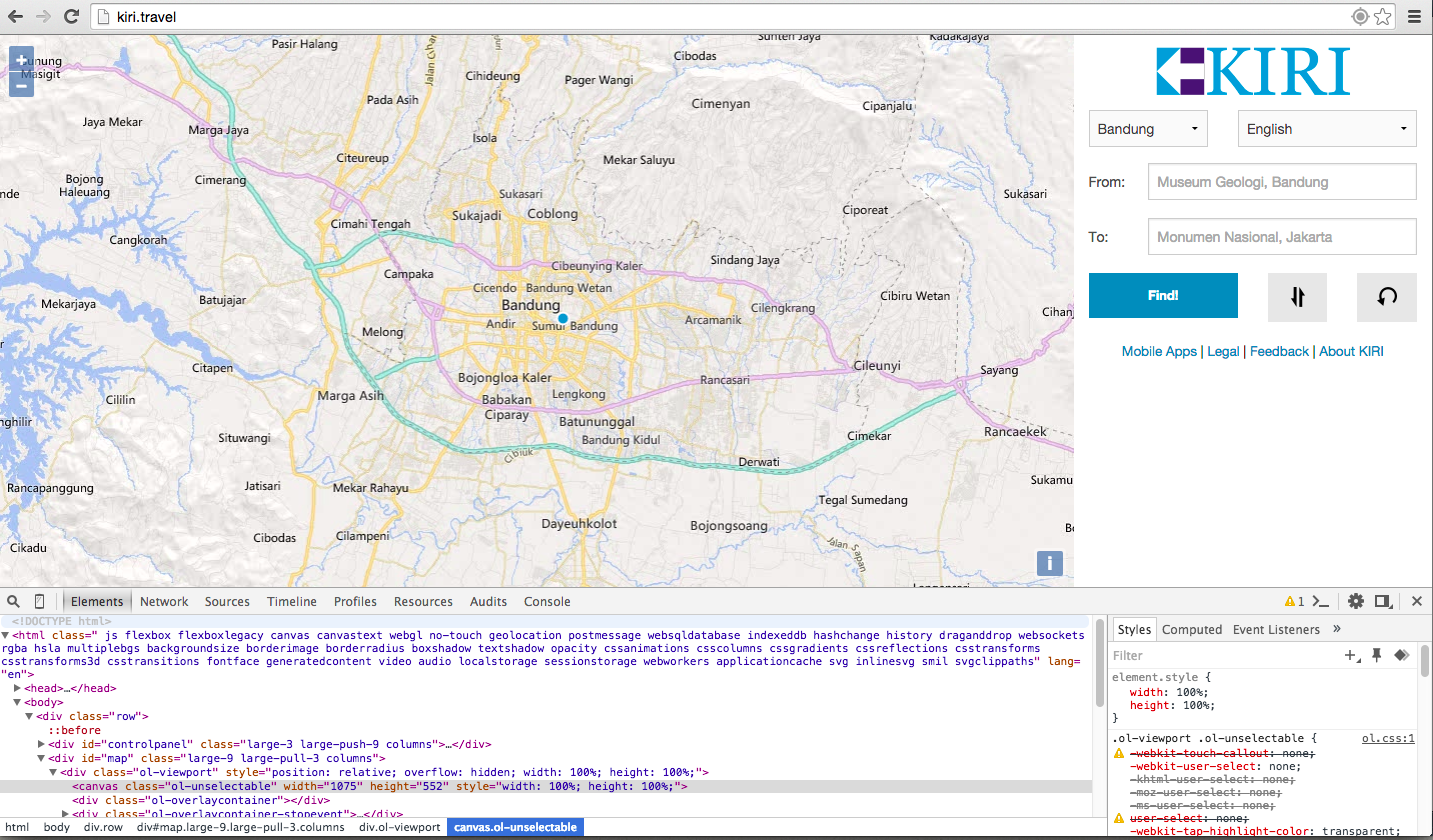
\includegraphics[scale=0.3]{Gambar/devtools-elements}
	\caption{Panel Elements} 
	\label{fig:2_devtools_elements}
\end{figure}

\subsection{Network}
Panel Network memberikan informasi tentang sumber daya yang diminta dan sumber daya yang diunduh melalui jaringan secara \textit{real-time}. Panel Network juga memperlihatkan waktu yang dibutuhkan untuk permintaan sumber daya. Sebagai contoh pada gambar \ref{fig:2_devtools_network}, saat melakukan pencarian rute, panel Network memperlihatkan apa saja sumber daya yang diperlukan serta waktu yang dibutuhkan pada proses tersebut. Tiap sumber daya pada panel Network terdapat kolom:

\begin{itemize}
	\item \textbf{Name}, nama sumber daya.
	\item \textbf{Status}, kode status HTTP \textit{request}.
	\item \textbf{Type}, tipe sumber daya.
	\item \textbf{Initiator}, asal dari sumber daya yang diminta.
	\item \textbf{Size}, ukuran sumber daya.
	\item \textbf{Time}, waktu yang dibutuhkan dalam permintaan sumber daya.
\end{itemize}

\begin{figure}[H]
	\centering
	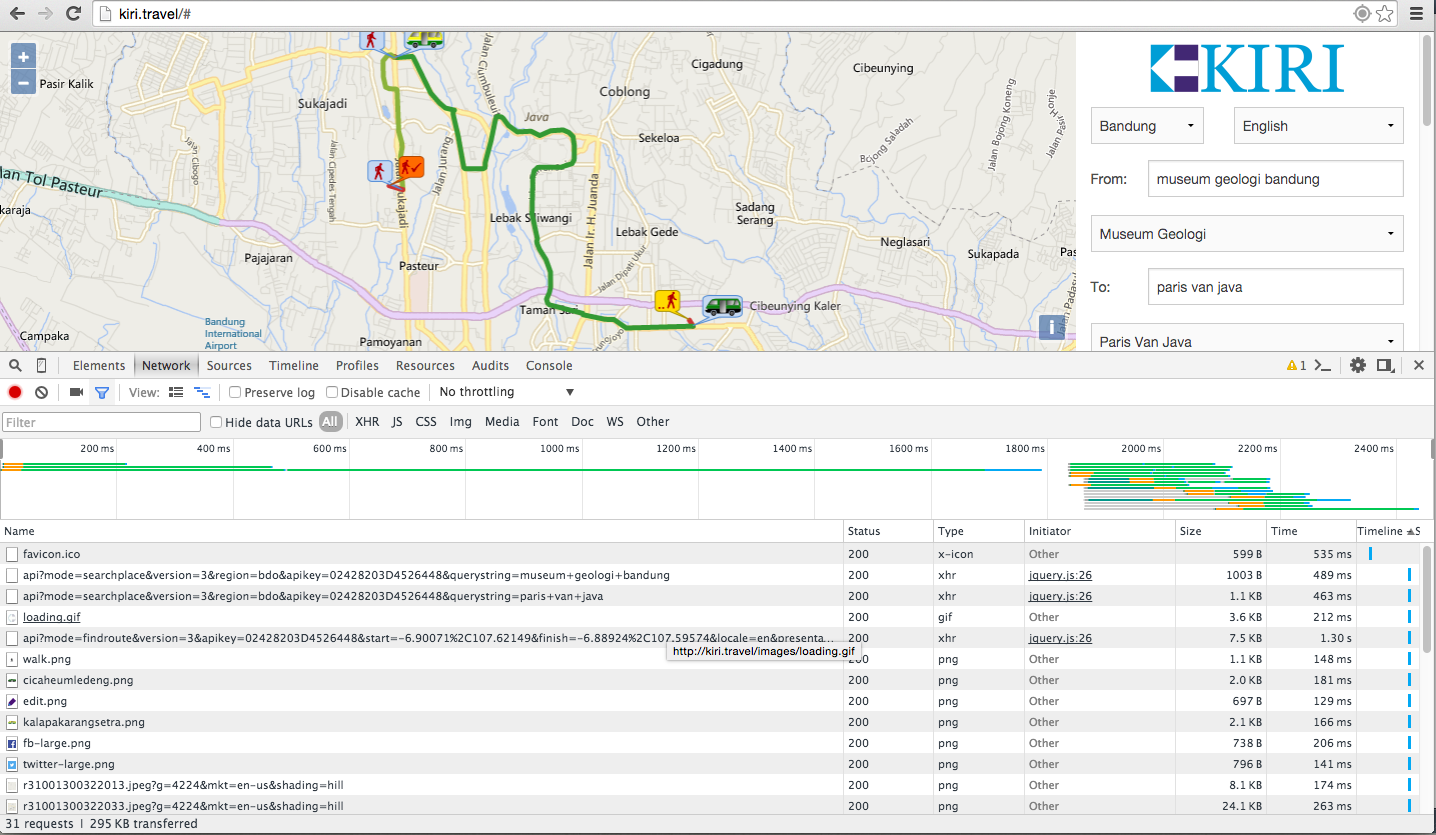
\includegraphics[scale=0.3]{Gambar/devtools-network}
	\caption{Panel Network} 
	\label{fig:2_devtools_network}
\end{figure}

Ketika sumber daya diklik, maka akan muncul bagian baru disamping sumber daya tersebut yang berisi kolom:
\begin{itemize}
	\item \textbf{Header}\\
			Header menampilkan \textit{request} URL, \textit{request method}, \textit{status code}, \textit{response headers}, \textit{request headers}, dan \textit{query string parameters} beserta nilainya.
			\begin{figure}[H]
				\centering
				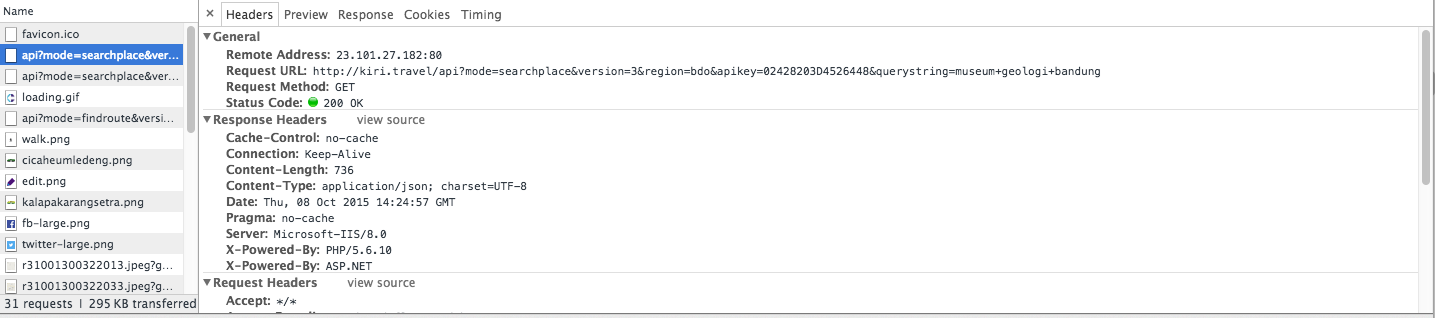
\includegraphics[scale=0.3]{Gambar/devtools-network-header}
				\caption{Contoh Header} 
				\label{fig:2_devtools_network_header}
			\end{figure}
	\item \textbf{Preview}\\
			Preview menampilkan peninjauan sumber daya jika sumber daya tersebut tersedia. Gambar \ref{fig:2_devtools_network_preview_a} menunjukkan adanya peninjauan sumber daya, sedangkan gambar \ref{fig:2_devtools_network_preview_b} menunjukkan tidak ada peninjauan sumber daya.
			
			\begin{figure}[H]
				\centering
				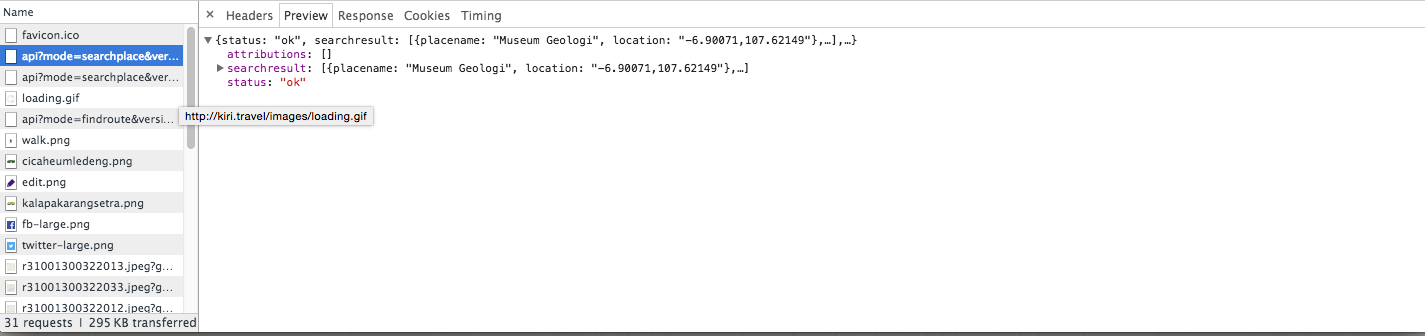
\includegraphics[scale=0.3]{Gambar/devtools-network-preview-a}
				\caption{Contoh peninjauan sumber daya tersedia} 
				\label{fig:2_devtools_network_preview_a}
			\end{figure}
			
			\begin{figure}[H]
				\centering
				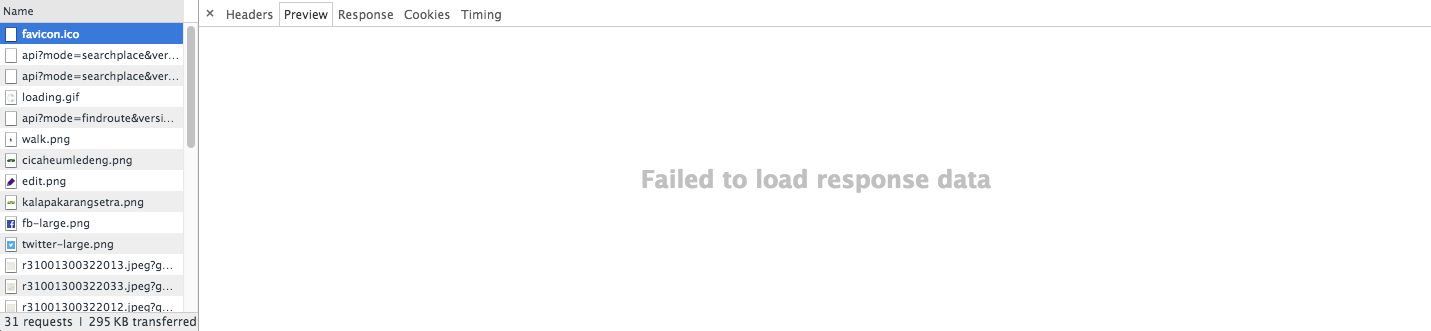
\includegraphics[scale=0.3]{Gambar/devtools-network-preview-b}
				\caption{Contoh peninjauan sumber daya tidak tersedia} 
				\label{fig:2_devtools_network_preview_b}
			\end{figure}
			
	\item \textbf{Response}\\
			Response menampilkan respon dari sumber daya yang dipilih. Gambar \ref{fig:2_devtools_network_response} menunjukkan respon dari sumber daya.
			
			\begin{figure}[H]
				\centering
				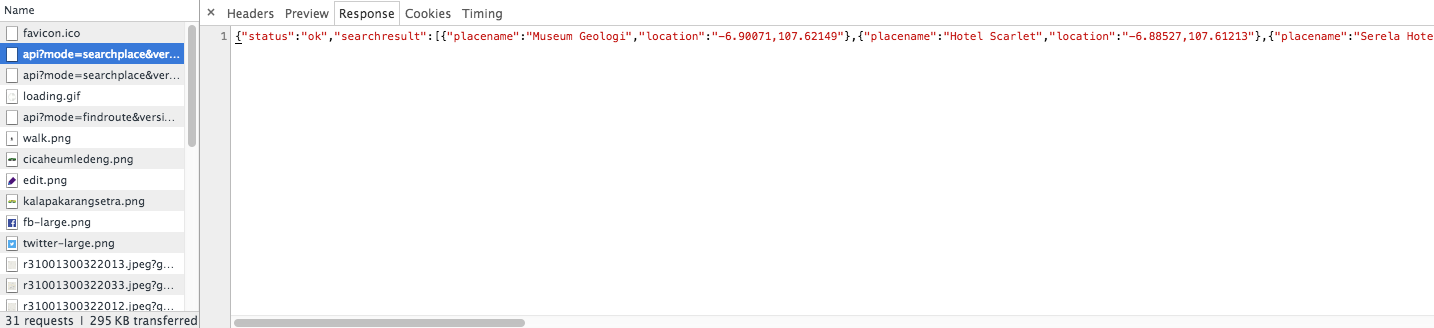
\includegraphics[scale=0.3]{Gambar/devtools-network-response}
				\caption{Contoh Response} 
				\label{fig:2_devtools_network_response}
			\end{figure}
			
	\item \textbf{Cookies}\\
			Cookies digunakan server web untuk menyimpan data pada \textit{browser} klien.  Kolom Cookies menampilkan seluruh \textit{cookie} yang terdapat pada halaman web. Pada gambar \ref{fig:2_devtools_network_cookies} terdapat kolom:
			\begin{itemize}
				\item \textbf{Name}, nama \textit{cookie}.
				\item \textbf{Value}, nilai \textit{cookie}.
				\item \textbf{Domain}, asal \textit{cookie}.
				\item \textbf{Path}, URL \textit{cookie}.
				\item \textbf{Expires / Max-Age}, batas habis \textit{cookie}.
				\item \textbf{Size}, ukuran \textit{cookie}.
				\item \textbf{HTTP}
				\item \textbf{Secure}
				\item \textbf{First-Party}
			\end{itemize}					 
			
			\begin{figure}[H]
				\centering
				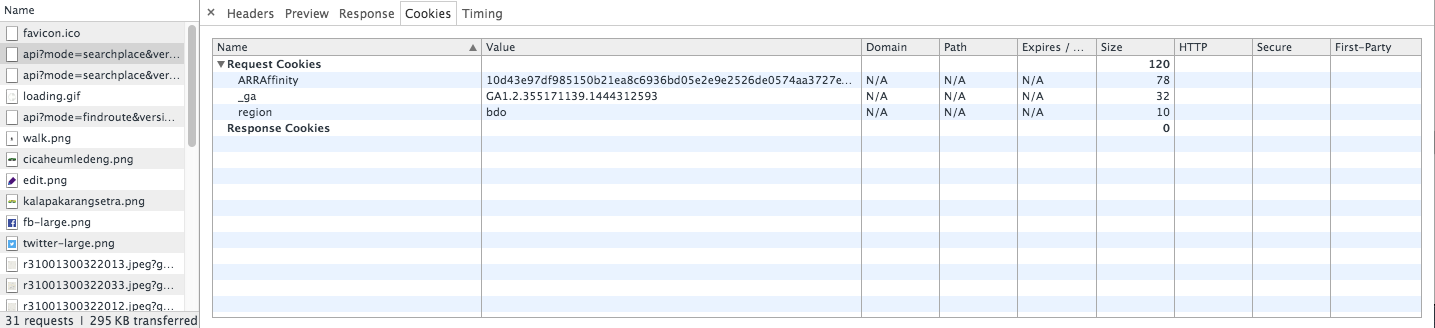
\includegraphics[scale=0.3]{Gambar/devtools-network-cookies}
				\caption{Contoh Cookies} 
				\label{fig:2_devtools_network_cookies}
			\end{figure}
\end{itemize}

\subsection{Sources}
Panel Sources memungkinkan untuk melakukan \textit{debugging} JavaScript dengan menggunakan \textit{breakpoints} \footnote{Terdapat dua cara untuk menambahkan \textit{breakpoints}. Cara pertama adalah Manual \textit{breakpoints}, yaitu mengatur \textit{breakpoints} pada baris kode. Cara kedua adalah Conditional \textit{breakpoints}, yaitu \textit{breakpoints} secara otomatis muncul ketika suatu kondisi terpenuhi, misal ketika \textit{on click}}. Pengembang membutuhkan alat \textit{debugging} untuk menemukan penyebab masalah dan memperbaikinya dengan cepat.

\begin{figure}[H]
	\centering
	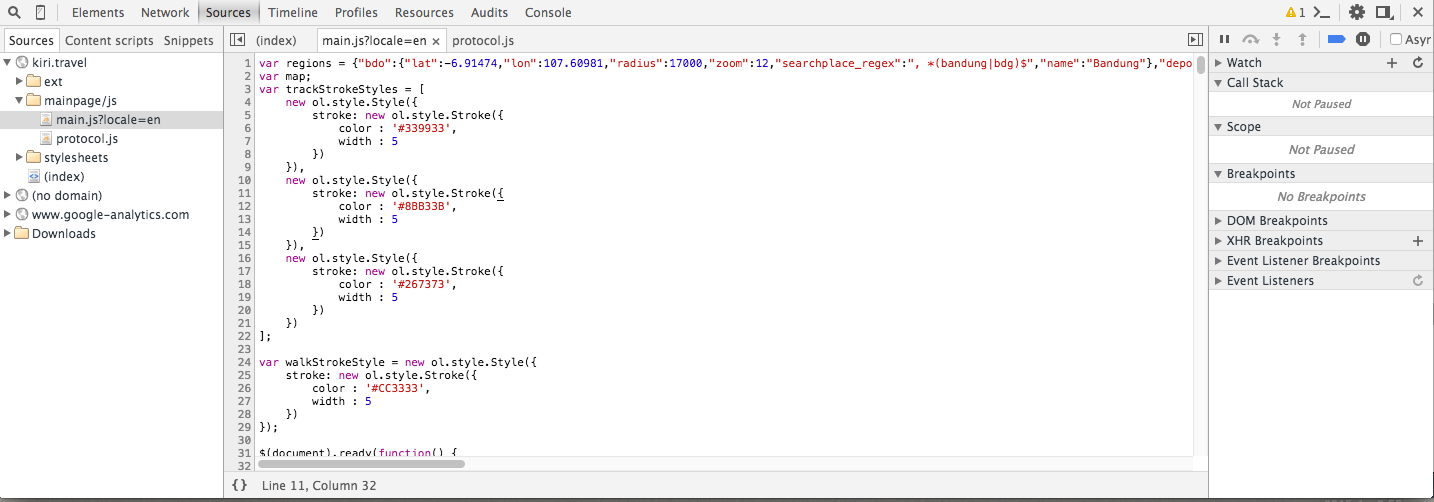
\includegraphics[scale=0.3]{Gambar/devtools-sources}
	\caption{Panel Sources dengan menyalakan Conditional \textit{breakpoints}} 
	\label{fig:2_devtools_sources}
\end{figure}

\subsection{Timeline}
Panel Timeline memberikan gambaran lengkap waktu yang dibutuhkan semua sumber daya yang dibutuhkan ketika memuat dan menggunakan halaman web. Sebagai contoh pada gambar \ref{fig:2_devtools_timeline}, panel Timeline memberikan gambaran lengkap ketika melakukan pencarian rute. 

\begin{figure}[H]
	\centering
	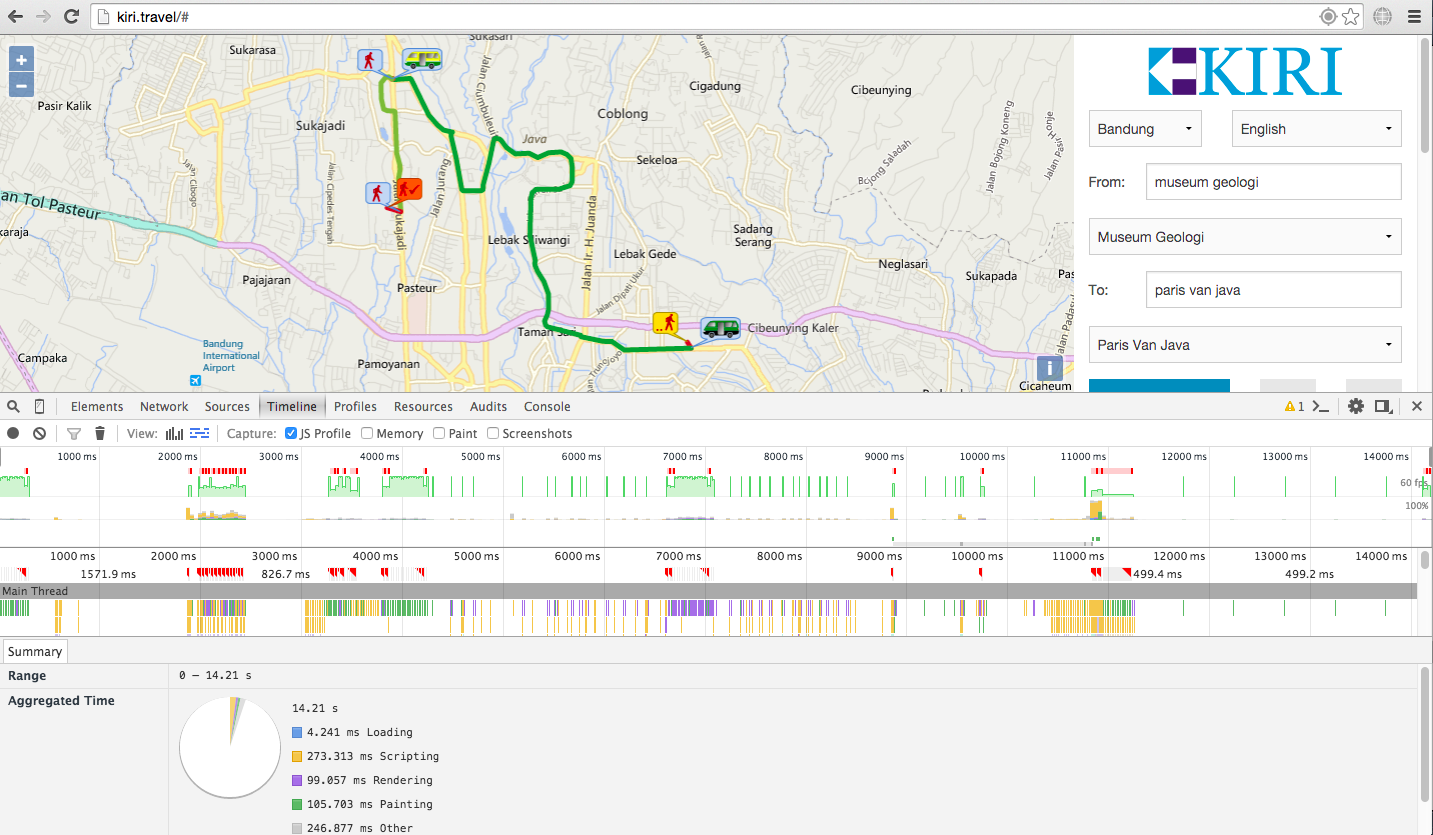
\includegraphics[scale=0.3]{Gambar/devtools-timeline}
	\caption{Panel Timeline saat melakukan pencarian rute} 
	\label{fig:2_devtools_timeline}
\end{figure}

\subsection{Profile}
Panel Profile memberikan riwayat waktu pelaksanaan dan penggunaan memori dari halaman web. Profile yang tersedia adalah:
\begin{itemize}
	\item CPU \textit{profiler} menunjukkan waktu eksekusi yang dihabiskan oleh fungsi JavaScript. Gambar \ref{fig:2_devtools_profile_cpu} menunjukkan waktu eksekusi yang dihabiskan oleh JavaScript.
			\begin{figure}[H]
				\centering
				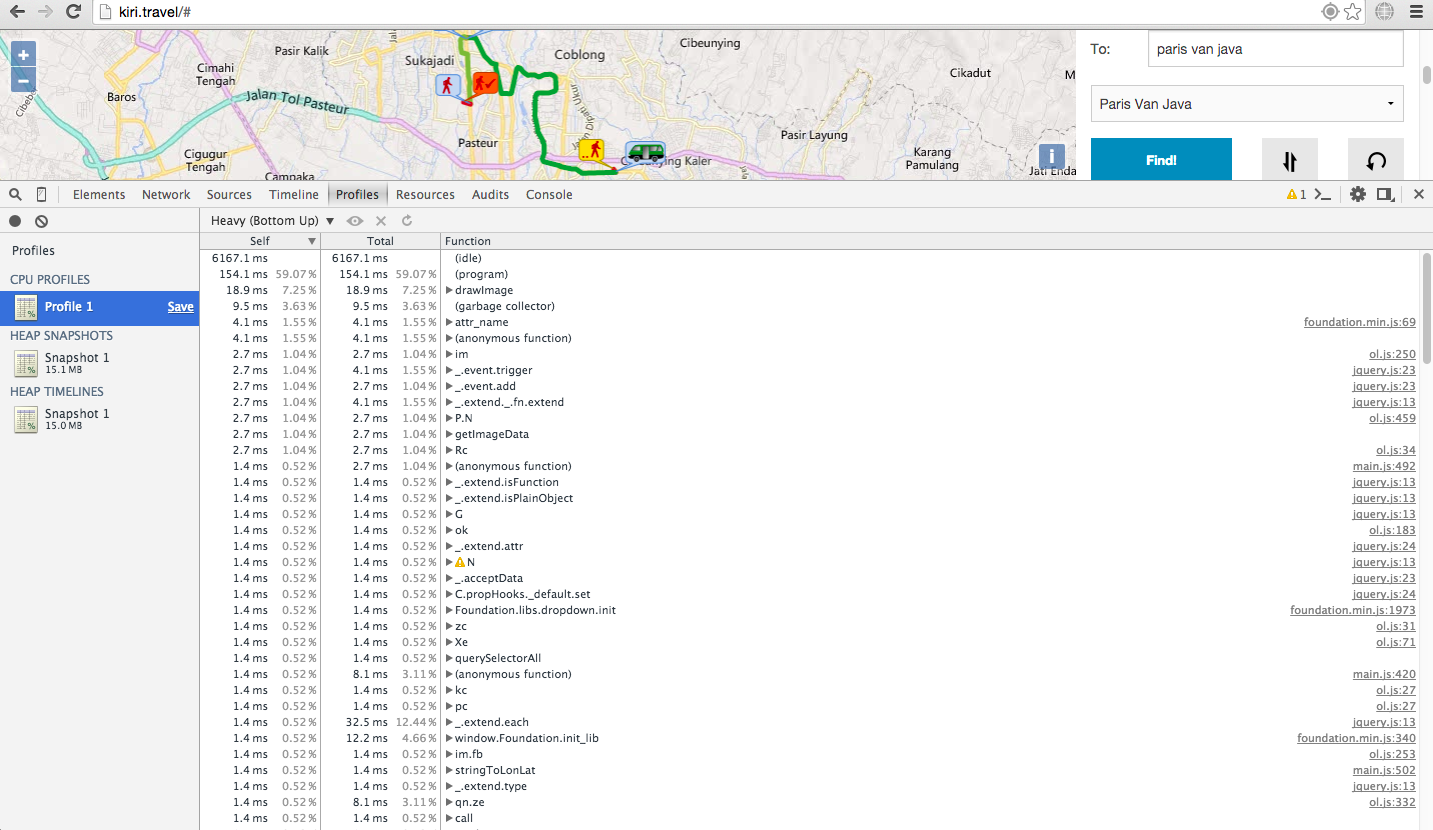
\includegraphics[scale=0.3]{Gambar/devtools-profile-cpu}
				\caption{Contoh CPU \textit{profiler}} 
				\label{fig:2_devtools_profile_cpu}
			\end{figure}
	\item Heap \textit{profiler} menunjukkan distribusi memori oleh JavaScript dan DOM yang berhubungan pada halaman web. Gambar \ref{fig:2_devtools_profile_heap} menunjukkan disribusi memori. 
			\begin{figure}[H]
				\centering
				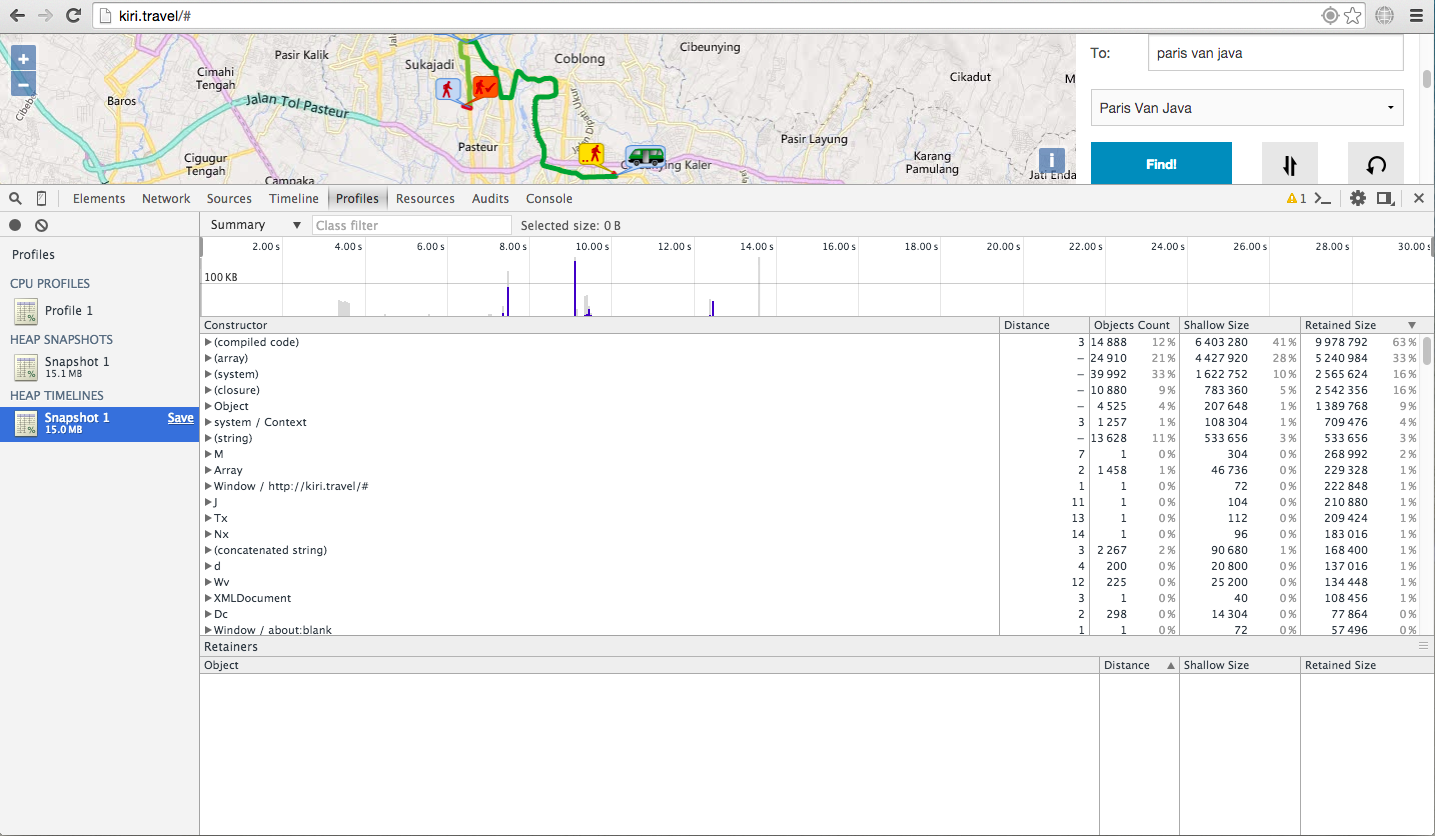
\includegraphics[scale=0.3]{Gambar/devtools-profile-heap}
				\caption{Contoh Heap \textit{profiler}} 
				\label{fig:2_devtools_profile_heap}
			\end{figure}
	\item JavaScript \textit{profiler} menunjukkan dimana waktu eksekusi dihabiskan pada skrip.
\end{itemize}

